\section{Results}
\label{sec:results}

\begin{figure*}[t]
  \centering
  \footnotesize
  \setlength{\tabcolsep}{3pt}
  \begin{tabular}{@{}*{3}{>{\centering\arraybackslash}p{0.322\textwidth}}@{}}
    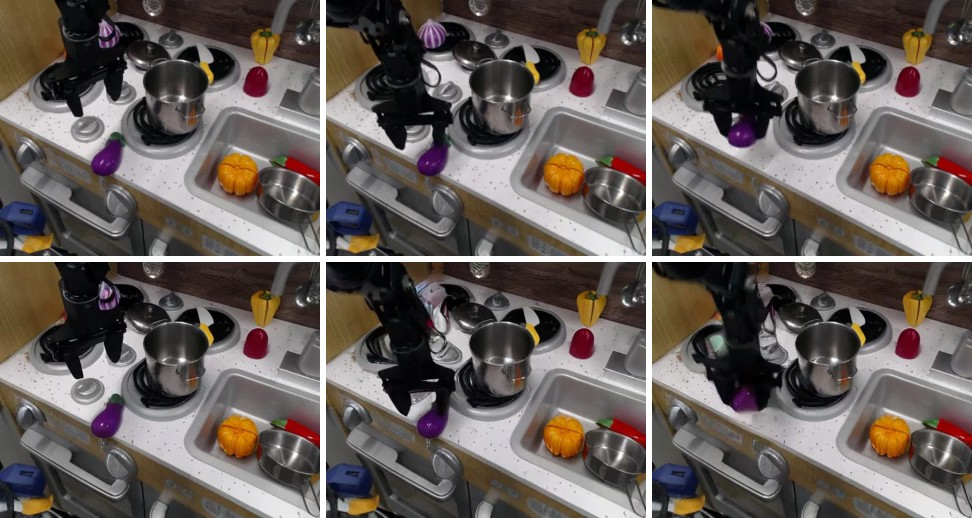
\includegraphics[width=0.322\textwidth]{fig/strip_13_0_0.jpg} &
    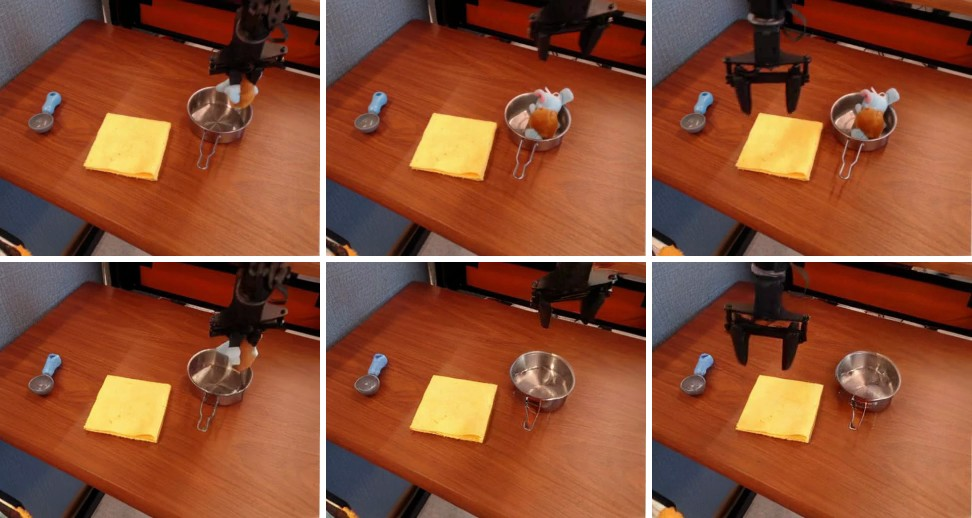
\includegraphics[width=0.322\textwidth]{fig/strip_6_0_32.jpg} &
    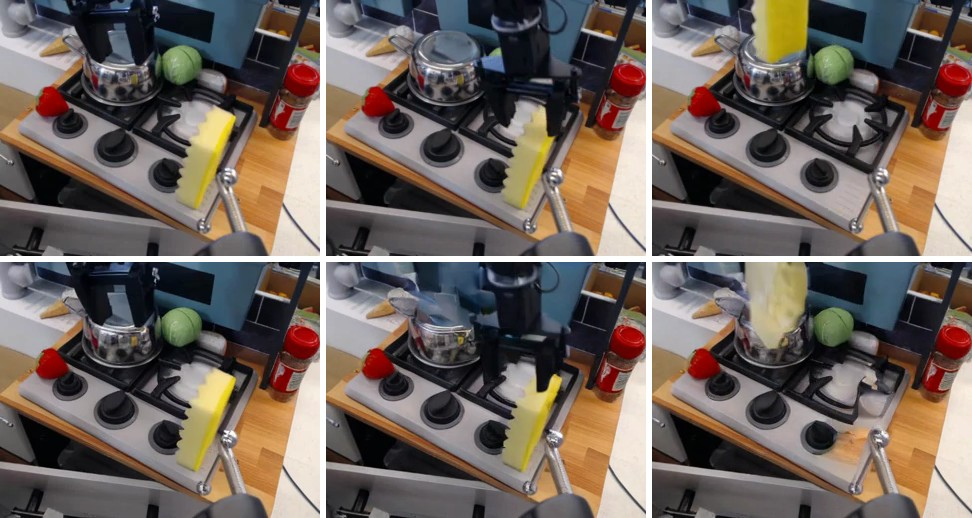
\includegraphics[width=0.322\textwidth]{fig/strip_1183_0_0.jpg} \\
    (a) ``put eggplant in pot'': success &
    (b) ``put the toy in the vessel'': the toy vanishes &
    (c) ``wipe pot with sponge'': the sponge breaks up \\
    PSNR 23.85, EVID 1.04 vs 1.00\,cm &
    PSNR 24.01, EVID 3.28 vs 2.52\,cm &
    PSNR 21.90, EVID 2.59 vs 1.80\,cm \\
  \end{tabular}
  \caption{Frames 0, 8, and 15 of the real video (top) and of IRASim-Frame-Ada from the same actions (bottom); both judges agree on each verdict. EVID errors of the generated and the real video. Both object failures raise the EVID error by less than 1\,cm, and PSNR rates (b) highest: the judges see these failures, neither metric does.}
  \label{fig:strips}
\end{figure*}

\begin{table}[t]
  \centering
  \footnotesize
  \setlength{\tabcolsep}{2pt}
  \begin{tabular}{@{}lcccccc@{}}
    \toprule
    & \multicolumn{3}{c}{Appearance} & 2-D & \ours{} & Paper \\
    \cmidrule(lr){2-4}\cmidrule(lr){5-5}\cmidrule(lr){6-6}\cmidrule(l){7-7}
    Model & PSNR$\uparrow$ & SSIM$\uparrow$ & LPIPS$\downarrow$ & NDTW$\uparrow$ & cm$\downarrow$ & PSNR$\uparrow$ \\
    \midrule
    \multicolumn{7}{@{}l}{\textit{Bridge, 105 clips}} \\
    IRASim-Frame-Ada & \ul{23.87} & \ul{0.808} & \ul{0.083} & \ul{0.709} & \ul{1.82} & \textbf{25.28} \\
    IRASim-Video-Ada & 23.52 & 0.804 & 0.087 & 0.682 & 1.95 & \ul{24.73} \\
    LVDM & 22.62 & 0.788 & 0.103 & 0.593 & 2.54 & 23.55 \\
    Cosmos-Predict2.5 & \textbf{25.74} & \textbf{0.859} & \textbf{0.063} & \textbf{0.754} & \textbf{1.64} & - \\
    \textit{Real video} & - & - & - & 1 & 1.50 & - \\
    \textit{Still video} & 19.80 & 0.805 & 0.141 & 0.156 & 9.06 & - \\
    \midrule
    \multicolumn{7}{@{}l}{\textit{Language-Table, 57 clips}} \\
    IRASim-Frame-Ada & \textbf{27.15} & \ul{0.861} & \textbf{0.059} & \textbf{0.702} & - & \textbf{28.82} \\
    IRASim-Video-Ada & 23.04 & 0.833 & 0.104 & 0.304 & - & 23.89 \\
    LVDM & \ul{26.44} & \textbf{0.863} & \ul{0.066} & \ul{0.646} & - & \ul{28.25} \\
    \textit{Still video} & 22.35 & 0.879 & 0.103 & 0.131 & - & - \\
    \bottomrule
  \end{tabular}
  \caption{Main results, frames 1 to 15. 2-D: NDTW of the end-effector track, 96 Bridge clips; \ours{}: EVID error, no reader for Language-Table; Cosmos-Predict2.5 with actions; Frame-Ada: mean of two seeds (std at most 0.17\,dB PSNR, 0.03\,cm); Paper: PSNR reported in~\cite{zhu2024irasim} on its full test set. Best in bold, second underlined, references in italics excluded.}
  \label{tab:bridge}
\end{table}

\begin{table}[t]
  \centering
  \footnotesize
  \setlength{\tabcolsep}{3pt}
  \begin{tabular}{@{}lcccccc@{}}
    \toprule
    & \multicolumn{3}{c}{Appearance} & 2-D & \multicolumn{2}{c}{\ours{}} \\
    \cmidrule(lr){2-4}\cmidrule(lr){5-5}\cmidrule(l){6-7}
    Actions & PSNR$\uparrow$ & SSIM$\uparrow$ & LPIPS$\downarrow$ & NDTW$\uparrow$ & cm$\downarrow$ & Exec. \\
    \midrule
    Original & \textbf{23.95} & \textbf{0.809} & \textbf{0.082} & \textbf{0.699} & \textbf{1.81} & 99.0 \\
    Noise 0.5\,cm & \ul{21.65} & \ul{0.782} & \ul{0.107} & \ul{0.557} & \ul{2.57} & 99.0 \\
    Noise 1.5\,cm & 18.93 & 0.744 & 0.152 & 0.256 & 5.46 & 99.0 \\
    All zero & 19.01 & 0.748 & 0.160 & 0.170 & 8.88 & 100 \\
    Mirrored & 18.22 & 0.730 & 0.179 & 0.093 & 14.56 & 93.3 \\
    \textit{Still video} & 19.80 & 0.805 & 0.141 & 0.156 & 9.06 & 100 \\
    \bottomrule
  \end{tabular}
  \caption{Perturbation test: IRASim-Frame-Ada on the 105 Bridge clips from corrupted actions, scored against the real clip of the original actions. Exec.: \% of clips executable by the WidowX 250, a necessary condition, not ranked.}
  \label{tab:perturb}
\end{table}

\subsection{Reproduction and model comparison}
Among the IRASim models, Frame-Ada leads on every metric, Video-Ada is second, and LVDM third, with significant differences on PSNR, 2-D NDTW, and \ours{} (\cref{tab:bridge}); Language-Table gives the same order, except that Video-Ada falls far behind, as in the paper.
Cosmos-Predict2.5 with actions has the best mean on every metric and a significantly higher PSNR, 1.9\,dB above Frame-Ada; its EVID error of 1.64\,cm is within 0.14\,cm of the error on the real videos, the floor set by the reader.
SSIM hardly separates the IRASim models from the still video.

\subsection{Do the metrics notice wrong actions?}
We regenerate the 105 clips with Frame-Ada from corrupted actions (\cref{tab:perturb}).
NDTW and \ours{} degrade steadily with the corruption, place zero actions at the level of the still video, and mirrored motion beyond it; \ours{} does so without the real video.
SSIM rates the still video above every corrupted generation and as high as the correct one, and PSNR and LPIPS prefer it to the three strongest corruptions.

\subsection{Validating \ours{}}
On real videos the EVID error is 1.50\,cm (95\% interval 1.36 to 1.68) for clips that move 25\,cm on average, while a still video scores 9.06\,cm, as poorly as assuming no motion, so the reader uses the frames rather than a prior.
\ours{} grows monotonically with the corruption and ranks the models as the reference-based metrics do, each step being significant.
The executability check accepts 99\% of clips for every action-conditioned model, the only failure being a clip the reader misreads on the real video as well, and rejects 7\% of the mirrored ones: the arm motion of these models is almost always feasible, so executability is a necessary condition, and the EVID error is what separates the models.

\subsection{What \ours{} reveals}
Without actions, Cosmos-Predict2.5 produces smooth videos, with a DINOv2 adjacent-frame similarity of 0.916 against 0.952 for real ones, whose robot does not follow the recorded motion: on the 24-clip subset its EVID error of 10.30\,cm does not differ significantly from the still video's 9.52\,cm, against 1.74\,cm with actions, and it can even replace the WidowX by another robot arm.
Two vision-language judges, gemini-3.8-flash and gpt-6.1-sol, differ in strictness, flagging 32\% and 1\% of real clips; for every IRASim model they most often flag objects that change or vanish, in 47\% and 10\% of Frame-Ada clips, which neither \ours{} nor the appearance metrics detect (\cref{fig:strips}).
Keeping the sample with the lowest EVID error among six Frame-Ada seeds raises PSNR from 23.92 to 24.07\,dB and the 2-D NDTW from 0.720 to 0.736, small but significant gains on metrics that use the real video, which the selection does not; for PSNR this is a sixth of what an oracle selecting with the real video reaches.

% ---- review comments, kept for the record (text above rewritten for concision on 2026-11-02) ----
% (Turn 5) "($p<10^{-7}$)", "($p<0.05$)", ...: You did not explain what is p here, and I am concern that is it necessary to calculate the p here? What does it represent for? The same with paragraph "Language-Table, 57 clips"
% Claude: p is the p-value of a paired Wilcoxon signed-rank test over the same clips: the chance of seeing a difference this consistent across clips if the two models were in fact equally good. It is worth keeping the test, because several gaps here are small next to the clip-to-clip spread (0.18 cm against a 1.5 cm reader error) and with about 100 clips some gaps are chance; indeed Cosmos's lead on NDTW and EVID turns out not to be significant. But you are right that listing p everywhere is unusual: the reference papers report none (Physics-IQ shows a 95% confidence interval). So p is now defined once in Sec. 4 ("significant" means p < 0.05) and the results just say significant or not.
% (Turn 5) "with seed 3407 (p = 0.017) but not with seed 3408 (p = 0.09)": I don't think in professional paper they also write in too much details like this, check reference papers to see how they write their papers
% Claude: agreed; IRASim and the other references report means only. Per-seed detail is gone; where a result does not hold for both seeds the text says "not significant" or "less clearly".
% (Turn 5) I do not see you mention about our metric EVID here? I just found the term "the cycle error" only
% Claude: agreed; the results now name EVID throughout ("the EVID error" for the cm value, "executability" for the check), and the tables' 3-D columns are labelled EVID.
% (Turn 5) "[20] reports the same gap, 23.89 dB for Video-Ada against 28.25 for LVDM and 28.82 for Frame-Ada, so it is a property of the model rather than of our run. ": You write like you are talking to me, not writing a professional paper 
% Claude: agreed; rewritten in report style, and the three numbers are left to the "Reported" column of Tab. 4.
% (Turn 5) " the 24 core clips": When the extra experiments on 105 clips done, replace all 24-clips' numbers in this paper by new 105-clips' numbers for unification!
% Claude: done wherever 105-clip data exists: the perturbation test (new A100 run), temporal consistency, the model ranking by EVID, and the analysis section. One result changed: on 105 clips SSIM rates the static video as high as, not above, the correct generation; abstract, intro, conclusion and slides now say so. Three parts stay on 24 clips because they were not run on 105 and need more GPU or API time than is left: the model without actions (3 min per clip on an A100), six seeds for best-of-N, and the two judges; each says "24 clips" explicitly.
% (Turn 6) This paragraph has too many numbers, which is too hard to follow for readers
% Claude: agreed; the paragraph is now organised as four checks with one key number each. Moved out (kept in reading_guide.md for the defence): per-axis correlations 0.88 to 0.93, gripper balanced accuracy 0.87, the bootstrap interval, the 27 to 29% of clips where a generated video scores better than its real video, and the correlation values.
% (Turn 6) How do you check if a clip is executable? If executable is just simply that the WindowX 250 6-DoF  robot can perform the action trajactories, so does this experiment make any sense? Should we remove it or use another checking mechanism?
% Claude: How: inverse kinematics of the WidowX 250 for each of the 16 poses read from the video, then joint limits and joint speeds between frames (Sec. 5). Does it make sense: yes, as a necessary condition, and I recommend keeping it in this shortened form. (1) It is the only measurement in the report of the brief's third question, whether generated motion is executable; removing it would leave that question unanswered. (2) Its answer is informative even though it barely separates the models: the arm motion of current models is feasible, so their failures are in action following and objects, not in impossible arm motion. (3) It does react to grossly wrong motion (mirrored actions). Its limit is now stated in the first sentence. A stronger mechanism is replay in a physics simulator of the same robot (SIMPLER), which adds dynamics, contacts and collisions; it needs a new environment and cannot be done reliably before 18:00, so it stays as the next step in the conclusion and slides.
% (Turn 7, chat) Fig. 2 (Spearman correlation matrix): why are 2-D NDTW and 3-D EVID treated as one group when they correlate weakly? What does this matrix mean, does it highlight our contribution? If not, remove it.
% Claude: you are right, removed (figure, sentence, and its script). (1) The grouping was by what the metrics measure (end-effector motion), not an empirical cluster; the data do not support a cluster (EVID vs NDTW 0.54, about the same as EVID vs appearance, 0.48 to 0.59). (2) A per-clip correlation cannot say why two metrics disagree: the reader floor of EVID (1.50 cm), CoTracker errors, the depth that a 2-D track cannot see, and the different references (commanded actions vs real video) all lower it, so a moderate value neither supports nor refutes EVID. (3) Its only clear message, that PSNR, SSIM, and LPIPS are redundant (0.84 to 0.95), is known and is not our contribution. The evidence for EVID is the floor and still-video bounds, the monotonic response in the perturbation test, and the agreement of the model ranking, all in Sec. 6.
